\documentclass{article}

\usepackage{fullpage}
\usepackage[utf8]{inputenc}
\usepackage{listings}
\usepackage{caption}
\usepackage[svgnames]{xcolor}
\usepackage{amssymb}
\usepackage{amsmath}
\usepackage{fancyhdr}
\usepackage{lastpage}
\usepackage{parskip}
\usepackage{abstract}
\usepackage{url}
\usepackage{float}
\usepackage{enumitem}
\usepackage{amstext}
\usepackage{fancybox}
\usepackage{amsmath}
\usepackage{graphicx}
\usepackage{subfigure}
\usepackage[bottom]{footmisc}
\usepackage{hyperref}
\usepackage{tikz}
\usepackage{makecell}
\usepackage{tabulary}
\usepackage{pdfpages}

\setcounter{secnumdepth}{5}

%%% Local Variables:
%%% mode: latex
%%% TeX-master: "report"
%%% End:

\newcommand{\code}[1]{\texttt{#1}}

%% source / reference
\newcommand{\refgeneral}[3]{#1 (#3), \emph{#2}}

% arguments:
%   author
%   title
%   year
%   publisher
\newcommand{\refbook}[4]{\refgeneral{#1}{#2}{#3}, #4}

% arguments:
%   author
%   title
%   year
%   url
\newcommand{\refonline}[4]{\refgeneral{#1}{#2}{#3} \\\url{<#4>}}

% pseudo code environment
\lstset{
  keywordstyle=\color{blue},
  commentstyle=\color{ForestGreen},
  stringstyle=\color{Maroon},%
  basicstyle=\ttfamily\small,
  frame=single,
  framesep=10pt,
  xleftmargin=30pt,
  xrightmargin=30pt,
  showspaces=false,
  showstringspaces=false,
  tabsize=4,
  aboveskip=10pt,
  belowskip=10pt,
  lineskip=2pt,
  numbers=left,
  numberstyle=\tiny,
  stepnumber=1,
  numbersep=5pt,
  breaklines,
}

\lstnewenvironment{pseudo}[1]{%
\lstset{morekeywords={if, then, else, return, function, var, for, foreach, do, end}}}%
{}

\pagestyle{fancy}
\fancyhf{}
\setlength{\parindent}{0pt}
\setlength{\headheight}{15pt}
\setlength{\headsep}{25pt}
\lhead{02122 Software Technology Project}
\rhead{The Kite Programming Language}
\cfoot{Page \thepage{} of \pageref{LastPage}}

\begin{document}

%%% Local Variables:
%%% mode: latex
%%% TeX-master: "report"
%%% End:

\newcommand*\formatname[2]{
  \leavevmode
  \rlap{\textit{#1}}
  \hspace{0.3\linewidth}
  \code{#2}}

\begin{titlepage}

\thispagestyle{empty}

\begin{flushright}
  
\includegraphics[width=9cm]{images/dtu}
\end{flushright}

\vskip20mm
\begin{center}
  
\includegraphics[width=3cm]{images/logo-clean}\\
  \vskip5mm
  \huge\textbf{The Kite Programming Language}
  \vskip5mm
  \Large 02122 Software Technology Project
  \vskip3mm
  \large June 2014
\end{center}
\vfill

\begin{flushleft}
  \normalsize
  \formatname{Simon Altschuler}{s123563} \par
  \formatname{Markus Veie Færevaag}{s123692} \par
  \formatname{Christian Mathias Rohde Kiær}{s123812} \par
  \formatname{Patrick Gadd}{s113491} \par
  \vskip2cm
  
\includegraphics[width=7cm]{images/dtu-compute}
\end{flushleft}

\end{titlepage}

\clearpage

\section*{Abstract}
%%% Local Variables:
%%% mode: latex
%%% TeX-master: "../report"
%%% End:

\clearpage

\tableofcontents
\clearpage

\section{Introduction}
%%% Local Variables:
%%% mode: latex
%%% TeX-master: "../report"
%%% End:
TODO: 1-2 pages
\subsection{Programming languages and compilers in general}
TODO: Give a short description of a compiler.


Programming languages are the means for programmers to express what the machine should compute, or in other words: What a program should do.
The two main divisions between programming languages are likely whether they are High- or Low-level and which `programming paradigm' they follow (in the next section these paradigms will be shortly described).

The low-level languages are close to what the computer `natively` understand, which is machine code/instructions, but are harder for humans to read and write. Examples hereof are FOTRAN and COBOL. Usually high-level languages are used for faster development, better readability and maintenance, among other things. Thus it is of general interest... SOMETHING SOMETHING


TODO: Describe paradigms in the next subsection

A programming language is implemented via a compiler

\subsection{Functional programming languages}
TODO: Give a short description of functional languages.


Terms to be described:
\begin{itemize}
\item Expressions
\item Higher order functions
\item Partial application
\item Currying
\item No mutable state
\item Not using statements (i.e. no side effects)

\end{itemize}

\subsection{The problem}
In short, we want to make our own functional programming language, Kite, by implementing a compiler.


Kite will feature the basic elements of most functional languages (described above), and a few additional features:

\begin{itemize}

\item Static typing and thus typechecking
\item Closures
\item If-expressions (not to be confused with if-statements)

\end{itemize}

\subsection{The structure of the report}
TODO

\clearpage

\section{Problem analysis}
\label{sec:probanal}
\subsection{Purpose of the project}
Our project is not concerned with solving a specific problem related to compilation of functional programming languages. Rather it is a project in which we aim to gain a thourough understanding of modern compiler theory and implementation as well as become proficient with functional development. We have made an effort to implement the compiler using modern techniques. That said, a compiler is a very complex piece of software and given our limited time, it is far beyond our scope to implement a language that could be used for production purposes. What we are striving for is a working language with all the elements of a basic functional language, expressive syntax, simple optimizations and target language that we can execute.

There are two main aspects of the project, one is that of functional programming language theory and design, the other is that of compiler implementation and techniques. Though they are very intertwined in the implementation we will often touch on the two aspects separately.

Next we will describe some properties of functional languages and compilers that we would like to implement in Kite. Further we will introduce some of the notation used throughout the rest of the report.

\subsection{Functional language properties}
We will describe function types using the following notation; let $f$ be a function with one parameter of type $Int$ (integer) and return value $Float$. We denote this using $:$, meaning ``of type'' or ``has type''

\[ f: Int \to Float \]

Note that the concrete types are capitalized, and we use small letters to indicate type variables, also known as polymorphic types. For instance $f: a \to b$ denotes a function which takes any type $a$ to any type $b$, and $f: a \to a$ denotes a function that takes any type $a$ and produces \emph{the same} type $a$.

The function operator $\to$ can be chained for a function to accept multiple parameters which we indicate as $f: a \to b \to c$. It's important to note that $\to$ is a \emph{binary} and \emph{right-associative} operator, meaning that

\[ f: a \to b \to c \quad = \quad f: a \to (b \to c) \]

This effectively means that a function always takes exactly one argument and produces one other. In the example above the returned value is a new function with type $b \to c$, which can then be applied to a value of type $b$ producing a final value of type $c$.

If we group the function operator differently we can describe functions that take other functions as argument. Consider for example $f: (a \to b) \to c$, indicating that $f$ takes a function of type $a \to b$ and returns a value of type $c$. The possibility to apply functions to functions and produce functions as return values is known as ``higher-order'' functions.

Closely related is the concept of functions as so-called ``first-class citizen'', which basically means that a function can be passed around and transformed just like any other value type.

We consider all functions to be \emph{anonymous}, meaning that they do not have a name associated with them in their definition. They can then be found to names using the \emph{bind} operation (syntactically denoted $=$) The following are examples of how we define concrete implementations of functions (later we will use Kite specific syntax, but for now we stick with simple mathematical notation)

\begin{align*}
id &= \fn{x}{x} & \text{The identify function, returns the argument unchanged}\\
add &= \fn{ x, y }{ x + y }  & \text{Add two values}\\
max &= \fn{ x, y }{ \ite{x > y}{x}{y} }  & \text{Calculate the maximum of two values}\\
\end{align*}

Here we use the $\lambda$ notation for functions using the ``maps to'' operator $\mapsto$ to indicate concrete implementation. We indicate function application using standard parenthesis, for instance $sum = add(2, 5)$.

A very powerful concept that rises naturally from that of higher-order functions, is that of partial application and currying. With partial application it is possible to apply a single argument to a function with multiple arguments, which produces a new function that accepts the remaining arguments. For instance, given the function $add$ from above, we can create a new function 

\begin{align*}
increment &: Int \to Int\\
increment &= add(1)
\end{align*}

which will take an $Int$ and add $1$ to it. Currying is closely related, but is concerned with transforming a function of type $f : a \times b \to c$ to the function $f' : a \to b \to c$, thus enabling partial application. Here we used another notation, namely $\times$ which denotes the Cartesian product of two values, which we will further describe as a \emph{pair} of values.

As can be observed from the above, functional languages are closely related to lambda calculus, and can be seen as an extension of it. Common for them is that almost everything is regarded as an expression, meaning that everything conveys a \emph{value}. For instance, in imperative languages the \code{if} construct is a statement, controlling flow of execution, whereas in a functional language, it's a choice between two values.

When working in imperative language, mutation of variables is a core feature that is used in almost all parts of a program. In a functional language however, it's common that variables are not in fact variable in the sense of being mutable, but rather declarations of values. For instance, to calculate the sum of a list of numbers (pseudo-code)

\begin{pseudo}

// imperative style
function sum(nums) do
  var s = 0
  foreach num in nums do
    s = s + num
  end
  return s
end

// functional style
function sum(nums) do
  return if length of nums is 0
    then 0
    else head(nums) + sum(tail(nums))
end
\end{pseudo}

Here we can see how the imperative code continuously mutates the \code{s} variable, and the functional code instead leverages recursion (and also is an example of the previously mentioned \code{if} as an expression).

The idea of immutability is related to the strive for controlling side effects. In a purely functional language, a function will \emph{always} produce the same value, given the same input. This makes the code much easier to reason about, because one does not have to worry about what state a certain function is in at a given time. It can also help the compiler make optimizations, which we will discuss in more detail later. Pure languages are however not practical for writing useful programs because, for instance, IO is inherently not pure. You can't know in advance what input the user will give you, and a truly pure function cannot generate random numbers, get the time, etc. Solutions have been developed to keep a language pure while still maintaining side effecting operations such as IO. For instance Haskell uses the concept of Monads to force side effecting functions to declare which effects they might have and provide fallback strategies in case of failure.


\subsection{Implementing a compiler}

Most modern compilers are built using more or less the same architecture. The source code of the compiled language is first analyzed lexically (a process sometimes referred to as \textbf{lexing}) into a stream of lexical tokens. This can be compared to splitting a natural language text into a list of words. This stream of tokens is parsed into nodes in an Abstract Syntax Tree (AST) using a \textbf{parser}. This can again be compared to natural language by imaging a list of word and punctuation being parsed into phrases that have ``meaning''.

The AST can have various forms and structure, but common is that it is a representation of the source code in the form of data structures native to the language of implementation. The AST can be transformed for different purposes, for instance to give correct precedence to operators.

Going further it can be analyzed in many different ways, for instance to perform \textbf{type checking} and ensure that no undefined identifiers are referenced. It is also possible to perform various optimizations on the AST. Dead (unused) code can be detected and removed, common patterns of code can be transformen into a more effecient structure, functions can be inlined to remove the overhead of making a function call and much more. We will go into details about this later.

Finally the AST can be used to emit code for the target language of the compiler, process known as \textbf{code generation}. It worth noting that many different code generators can be implemented for the same AST, thus allowing to target multiple architectures and machines using the same compiler.

We are going to implement all of these modules, some more thouroughly than others, and in such a way that it can be easily extended and maintained.


%%% Local Variables: 
%%% mode: latex
%%% TeX-master: "../report"
%%% End: 

\clearpage

\section{Requirements}
\label{sec:requirements}
%%% Local Variables:
%%% mode: latex
%%% TeX-master: "../report"
%%% End:
In the requirements-section we will focus more on the language specific features of Kite. As most of the compiler specific requirements are discussed in the design-section, and are basic for most compilers, they will not be discussed here.

\subsection{Minimum requirements}
As of our initial requirements for Kite, we have set a list of minimum requirements for our compiler.

\textbf{Type system:} Standard types that should be included in Kite is as follows:
\begin{itemize}
\item [--] Float
\item [--] Integers
\item [--] Characters
\item [--] Boolean
\item [--] Lists
\item [--] Pairs
\end{itemize}

\textbf{Static type check:}
In our initial analysis, we want to implement a static type-checker. This will ensure type safety in a given program, i.e.\ a program passing the static type-check will be free of type errors. If a program is verified by the analyzer, the compiler will be able to trust the intermediate representation given from the type-checker. This will also result in any type error will be caught compile-time.

\textbf{Code generation:}
For a machine to be able to understand the high-level language, the process of code generation is needed. Kite's code generator must be able to take some representation of the given source code, and convert it such that the machine will be able to execute the resulting output.

\textbf{Recursion:}
As recursion is one of the main properties of a functional language, it will have to be a central aspect of Kite. In general, recursion is the method of dividing a problem into sub-problems. This is top-down approach to problem-solving and is commonly referred to as the technique ``divide and conquer''. A more specific example of recursion is a function calling it-self until one or more given base-cases are met. One of the most used examples of recursion is the computation of Fibonacci numbers. As a Fibonacci number is defined as the sum of the two previous numbers, it easily implemented with recursion (albeit this particular implementation is very inefficient):

\begin{pseudo}
// fibonacci
function fibonacci(n) do
  return if n < 2
    then n
    else fibonacci(n - 1) + fibonacci(n - 2)
end
\end{pseudo}


\subsection{Optional features}

\textbf{Standard library:}
Inspired by Haskell's prelude~\footnote{\url{http://hackage.haskell.org/package/base-4.7.0.0/docs/Prelude.html}}, we want to implement a standard function library, imported by default into all Kite modules. This standard module should include useful functions for common operations as arithmetic operations, string manipulations and list manipulation.

\textbf{REPL:}
A Read-Eval-Print-Loop, or an \emph{interactive top-level}, will allow a user to have a simple interactive program to give simple input, e.g. a single expression, evaluate it and get the return value, without creating an file and compiling it.

\textbf{Higher-order functions:}
The language should provide the possibility to create function that take functions as parameters, and returns functions.

\textbf{Immutability:}
In a pure functional language there will be immutability.
TODO


\textbf{Currying:}
As we want all functions only to take one parameter, we want to include currying.
TODO: Mention lambda calculus somewhere, Hindley Milner...

\textbf{Partial application:}
As a result of currying, we want to make use of partial application. E.i. construct the foundation of function in such a way that a function takes a fixed number of arguments, returning a new function of smaller arity~\footnote{The number of arguments or operands the function or operation accepts}.

\textbf{Closures:}
The principle of closures is that when a function is referenced, it is referenced together with a \emph{referencing environment}. This environment includes a table of all non-local variables of that function. This allows a function access to non-local  variables also when invoked outside its immediate lexical scope.

\textbf{Lazy evaluation:}
The language should include lazy evaluation, which will allow evaluation of expressions to be delayed until it's needed. This technique can greatly decrease the run-time of certain code patterns.

\textbf{Type inference:}
This is an extension of the type-checker. Type inference will let the analyzer automatically deduct types of expressions, thus removed the need to declaring the types of the parameters and return types of a function.

\textbf{I/O:}
Input/Output is needed for user interaction between the user and computer. To make the language more usable, a minimum of I/O must be present. Optional features would be read/write from file etc.

\textbf{Syntactic sugar:}
To make some expressions and code pattern more readable, we want to implement a sugaring module. With this module, features as list comprehension can be added (see below).

\textbf{List comprehensions:}
List comprehensions is syntactic sugar for creating new lists from already existing lists, which is an extension of syntactic sugaring. List comprehensions will output new lists, as a result of some operation performed on each element of another list (or lists). It should also be possible to create a sub-sequence of the elements of another list, by implying that each element in the created list should satisfy a number of conditions.

\textbf{Preprocessing:}
To make it possible to include another file into a given program, we want to make use of a preprocessor. The preprocessor should be C-like where '\#include' is used to specify which external files to be included. A simple preprocessor will suffice, like the C-preprocessor.


% Mutaddfdfbghnjghfhgrbhgfdghfdvfdgbhgfdghtdehgfhgfdfbgfdbility
% REPL
% StdLib
% HoF
% Rekursion
% String interpolation
% Closures
% Lazy eval
% Parallel
% Currying
% Type system (static, strong)
% *Type inference
% I/O
% “alt = expressions”
% List comprehension
% (else?)

% TODO:
% Language features:
% Conditionals
% Functions
% “let … in”
% Loops (boobs)
% Pattern matchin

% Typez:
% String
% List
% Int
% Float/double
% Tuples/structs

\clearpage

\section{Design of the Kite language}
\label{sec:kite-design}
We have been inspired by many other languages when designing and
implementing Kite, most notably the GHC Haskell compiler\footnote{The
  Glasgow Haskell Compiler \url{http://www.haskell.org/ghc}}.

\subsection{Syntax}

TODO: Sugar, List Comprehensions, describe types, more on function declaration.

Basic declaration of the variables in Kite, types are inferred by the analyzer:
\begin{kite}
  
  one = 1
  two = 2.0
  truth = True
  list = [1, 2, 3, 4]
  str = "foo" 
  pair = (1, "one")
\end{kite}

The basic types will be Int, Float, Bool, Lists, Chars and
pairs.

Functional languages often make extensive use of lists, which is
indeed also the case for Kite. A list is an ordered array of items
that can be transformed in many different ways. We use a common
short-hand method for describing a list of things, using square
brackets $[\ ]$. For instance, a $List(Int)$ (pronounced ``List of
Ints'') is denoted $[Int]$ and a list of a type variables $a$ is
$[a]$. Lists can be nested, allowing $List(List(Int))$ denoted
$[[Int]]$.

The pair type is also abbreviated using $(,)$, for instance the type
$Pair(Int, Bool)$ is written $(Int, Bool)$

Strings is represented as syntactic sugar for lists of characters,
which will be discussed later.

Basic arithmetic operators in Kite and their us
\begin{kite}

  two = 1 + 1  ---->  2
  str = "foo" ++ "bar" ----> "foobar"
  xor = 10 ^ 8 ----> 2
  mod = 10 % 2 ---> 0
\end{kite}

\begin{table}[H]
\centering
    \begin{tabular}{|l|l|}
    \hline
    Operation    & Meaning              \\ \hline
    x + y        & Additition           \\ \hline
    x - y        & Subtraction          \\ \hline
    x * y        & Multiplication       \\ \hline
    x / y        & Division             \\ \hline
    x**y         & Exponentiation       \\ \hline
    x \% m       & Remainder of x / y   \\ \hline
    pow(x, y, m) & Modulo exponentation \\ \hline
    \end{tabular}
\end{table}

Basic boolean operators:
\begin{kite}
  
  foo = 1 < 2  ----> True
  bar = 1 == 2 ----> False
  baz = 1 != 10 ----> True
\end{kite}
Basic boolean operators include 
\begin{table}[H]
\centering
    \begin{tabular}{|l|l|}
    \hline
    Operation & Meaning                 \\ \hline
    $==$        & equal                   \\ \hline
    $/\ =$        & Not equal               \\ \hline
    $<=$        & Less than or equal than \\ \hline
    $>=$        & Greater than or equal   \\ \hline
    $<$         & Less than               \\ \hline
    $>$         & Greater than            \\ \hline
    \end{tabular}
\end{table}

basic bitwise
\begin{kite}
  
  xor = 10 ^ 8 ----> 2
\end{kite}

TODO Conditional statements 
Function declaration in Kite:
Anonymous functions:

\begin{kite}
  
|ArgName, ... | -> { ... }
\end{kite}
Since all functions in Kite is anonymous, a function is simply a
variable bound to a given anonymous function. A function is declared
as follows:
\begin{kite}
  
  function :: ArgType, ... -> ReturnType
  function = |ArgName, ... | -> { ... }
\end{kite}
Example of valid function declaration in Kite, taking one parameter of
the type Int and returning an Int.
\begin{kite}
  
  foo :: Int -> Int
  foo = |a| -> {
    a + 1
  }
\end{kite}
A runnable program must always include a main function:
\begin{kite}
  
  main = -> { ... }
\end{kite}
Using a preprocessor to include another code file, use the \#include
keyword:
\begin{kite}
  
  #include "foo.kite"
\end{kite}

By using a sugaring module, Kite will be able to express certain
functions more clearly and readable. Syntactic sugar includes infix
operators, multiple parameters on function calls, list of characters
as strings and list comprehensions.

infix:
\begin{kite}
  
  foo = 1 + 2
\end{kite}

Desugar

\begin{kite}

  foo = ((+) (1)) (2)
\end{kite}

multiple parameters:
\begin{kite}
  
  foo = |a, b| -> {
    a + b
  }
\end{kite}
desugar:

\begin{kite}

  foo = |a| -> {
    return |b| -> {
      return ((+) (a)) (b)
    }
  }
\end{kite}
Strings 
\begin{kite}
  
  str = "Hello"
\end{kite}
Desugar:
\begin{kite}
  
  str = ["H", "e", "l", "l", "o"]
\end{kite}

\label{sec:ex-listcomp}
List comprehensions are syntactic sugar for manipulating
lists. An example of a list comprehension is as follows:
\begin{kite}
  
  list = [ x*y | x <- range(3,5), y <- range(4,6) | (x+y) >= 10, y > 4]
\end{kite}
where the desugared version of the same example, will look as follows:
\begin{kite}

  list =
  flatMap(|x| -> {
    flatMap (|y| -> {
      if (|x,y| -> {y > 4})(x,y) && (|x,y| -> {(x+y) >= 10})(x,y) 
         then [(|x,y| -> {x*y})(x,y)] 
         else []
    } , range(4,6) )
}, range(3,5) )
\end{kite}
Take note that list comprehensions uses functions defined in the
foundation, which will be discussed later
\subsection{Semantics}

TODO: Recursion, HoF, Currying, pattern matching,
partial application, Mutability. maaske mere.

Example of pattern matching
\begin{kite}

fibo = |a, b, n| -> {
    match n {
    0 -> a,
    n -> fibo(b, (a + b), (n - 1))
    }
}
\end{kite}

\subsection{Foundation}

As earlier mentioned, the foundation of Kite is a standard library
consisting of often used functions. Kites foundation is inspired by
Haskells prelude, and includes many functions found in prelude.
TODO: MORE FUN FUN FUN

%%% Local Variables: 
%%% mode: latex
%%% TeX-master: "../report"
%%% End: 

\clearpage

\section{Design of the compiler}
\label{sec:compiler-design}
%%% Local Variables:
%%% mode: latex
%%% TeX-master: "../report"
%%% End:

%%% TODO: move this to kite design
Functional languages often make extensive use of lists, which is indeed also the case for Kite. A list is an ordered array of items that can be transformed in many different ways. We use a common short-hand method for describing a list of things, using square brackets $[\ ]$. For instance, a $List(Int)$ (pronounced ``List of Ints'') is denoted $[Int]$ and a list of a type variables $a$ is $[a]$. Lists can be nested, allowing $List(List(Int))$ denoted $[[Int]]$.

The pair type is also abbreviated using $(,)$, for instance the type $Pair(Int, Bool)$ is written $(Int, Bool)$
%%%

To describe the overall design of the Kite compiler, we will start by
breaking it down into general parts, where each part or module has a
specific task. Below we have a waterfall model including the main
parts of the compiler:

\begin{figure}[H]
  \label{fig:flow}
  \center
  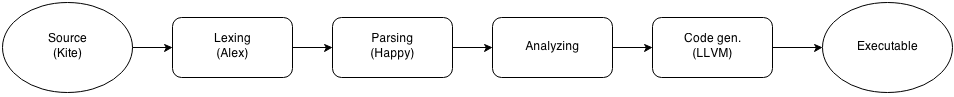
\includegraphics[scale=0.45]{images/flow.png}
  \caption{General flow of the Kite compiler}
\end{figure}

At first it can seem a little daunting, but when we get into the
purpose of each step, there will be a more obvious flow.

\subsection{Preprocessor}
The first thing the compiler does is preprocess the input, e.i. the
source code files, that it has been given. This is quite simply the
task of including all necessary files into one file. The files to be
included are declared in the top of the file.

\begin{figure}[H]
  \label{fig:preprocessor}
  \center
  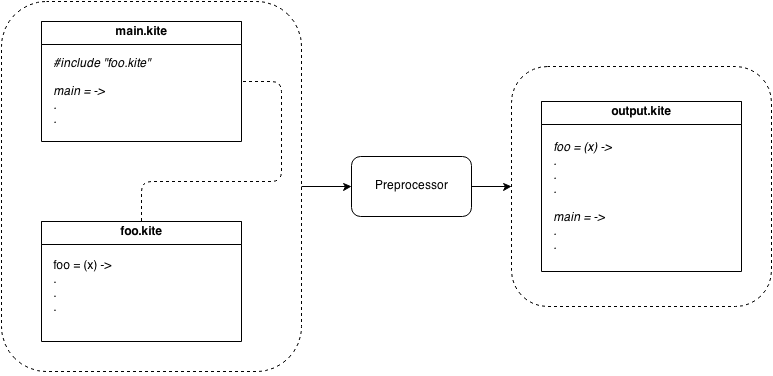
\includegraphics[scale=0.45]{images/preprocessor.png}
  \caption{Input and output of the Preprocessor}
\end{figure}

The nature of the preprocessor is quite simple, as the only task it
simple textual substitution.

\subsection{Lexical analysis}
The lexical analyzer, or just \emph{lexer}, is a central part of most
compilers. It has the important task of processing some input and
converting it to known, referencable tokens. This process is commonly
known as \emph{tokenization}.

Most lexers as quite simple, and does not contain much
complexity. That is often reserved for the parser and analyzer, which
we will come back to next.

\subsection{Parser}
The parser takes the string of tokens from the lexer, and based on a
language grammar, builds a corresponding data structure, namely the
parse tree. In the process it check that that the input is
syntactically correct. Therefor, this process is also called syntactic
analysis.

\subsection{Desugar}

\subsection{Analyzer}

\subsection{Optimizer}

\subsection{Code generation}
The code generator will take a representation of the
parse tree, the output of the parser, and generate code
accordingly. TODO: Inital, not done.

\clearpage

\section{Implementation}
\label{sec:impl}
TODO: Implementation of all 9 compiler-parts

\subsection{Preprocessor}

The preprocessor in Kite is almost identical to the \code{C} language preprocessor. We use a library called \code{cpphs}\footnote{\url{http://projects.haskell.org/cpphs}} that mimics the \code{C} version, and provides an embeddable Haskell library. This is the reason for the \code{\#include "file.kite"} syntax. Preprocessing is the first step of the compilation, and generates a single source code file which is a recursive concatenation of all included source files referenced from the main file.

\subsection{Lexer}
The lexer is implemented with the lexical generator Alex \cite{dornan01}. The lexer splits in

\subsection{Parser}
The parser is implemented with the LALR-parser generator Happy \cite{marlow01}. Happy automatically generates Haskell code from the file `src/Kite/Parser.y', which we have written in partially Haskell and partially Backus-Naur Form\footnote{This is a well known notation technique for specifying context-free grammars, which the more popular parser generator ANTLR also makes use of.}.

The current parser generates more than 2,000 lines of quite unreadable Haskell code, which is used in the compilation of the compiler. Fortunately Happy allows setting a --info flag when it is used, which also generates a .info-file about the parser. For instance it yields very useful information about shift-reduce and reduce-reduce conflicts, which has been a great throughout the development.

TODO (synes dette er lidt whack formuleret): `When a(/or a combination of) tokens are matched in the Parser, it is transformed into Haskell data-structures, from which we build the parse tree. TODO: Dette skal lede videre til syntactic zugar!


\subsection{Syntactic sugar}
\subsection{Analyser}

\subsubsection{Type inference}

As mentioned earlier, Kite uses static type checking to verify that types align at compile-time. We have used the Hindley-Milner type inference algorithm first described by Damas and Milner \cite{milner82}. They described an algorithm, named ``Algorithm W'', that given an expression will infer the most general type of that expression. We introduce the $\vdash$ to mean a derivation of types from an expression. For instance $x = 1 \vdash x : Int$ is read as ``given the expression $x = 1$ we can derive that $x$ has type $Int$''. To give a sense of what the algorithm does we first present a few examples. Recall that $:$ is pronounced ``has type''

Let the following be predefined
\begin{align*}
  +      & : a \to a \to a   \quad\text{(infix)}\\
  head   & : [a] \to a   \\
  fst    & : (a, b) \to a
\end{align*}

The algorithm can now infer the types of the following expressions
\begin{align*}
  \fn{xs}{head(xs) + 1} & \qcol [Int] \to Int    & \qvd xs : [Int]             \\
  \fn{p}{fst(p) + 1}    & \qcol (Int, a) \to Int & \qvd p : (Int, a)           \\
  f(n + 1)              & \qcol a                & \qvd f: (Int \to a), n: Int \\
\end{align*}

Using the last example above the intuition behind the algorithm is as follows

\begin{enumerate}
\item $e = \fn{f, n}{\ldots} \vdash e: (a \to b \to c)$ \\
  $e$ is being assigned a lambda expression with two parameters but we do not know anything about their types
\item $e = \fn{f, n}{f(\ldots)} \vdash f: d \to c$ \\
  $f$ is being applied to a single (yet unknown) value, thus we can infer that it is a function
\item $e = \fn{f, n}{f(n + 1)} \vdash n : Int$ \\
  We see that $f$ is applied to $n+1$ and since $1: Int$ and $+:a \to a \to a$ then $a = Int$ and thus $n:Int$ (this is called type unification, explained below).
\item $e = \fn{f, n}{f(n + 1)} \vdash e : (Int \to c) \to Int \to c$ \\
  There are no more expressions to infer so we end up with the final, most general type for $e$
\end{enumerate}

\paragraph{Type unification}

We define the $\tau$ function to ``type of'', such that for instance from the above $\tau(e) = (Int \to c) \to Int \to c$.

When the type of $n$ was inferred, we \emph{unified} the known type of $+:a \to a \to a$ with the expression $n + 1$. Note that $n + 1$ is equivalent to the prefix form $+(n, 1)$. From a base case (shown below) we know that $\tau(1) = Int = a$. This gives us

. This is called type unification and is at the core of the algorithm.

Formally the unification algorithm takes two types and either fails or returns a \emph{substitution} that maps the most general type to the most specific of the two. The algorithm is here formulated in Haskell code and is equivalent to that of our actual implementation (though simplified and not compilable)

\begin{haskell}[]
-- Note:
-- <+> is an infix function that composes (union) two substituions
-- nullSubst is an empty substituion

unify :: Type -> Type -> String -> TC Substitution

-- primitive base cases
-- empty substitutions
unify IntegerType IntegerType = return nullSubst
unify FloatType FloatType     = return nullSubst
unify CharType CharType       = return nullSubst
unify BoolType BoolType       = return nullSubst
unify VoidType VoidType       = return nullSubst

-- type var with any type
-- binds the type var name to the other type
unify ta (PTypeVar name) = varBind name ta
unify (PTypeVar name) tb = varBind name ta

-- list
unify (PListType ta) (PListType tb) = unify ta tb

-- pair
unify (PPairType ta tb) (PPairType ta' tb') = do
  sa = unify ta ta'
  sb = unify tb tb'
  return (sa <+> sb)

-- lambda
unify (PLambdaType paramA returnA) (PLambdaType paramB returnB) =
  sParam <- unify paramB paramA
  sReturn <- unify (apply sParam ra) (apply sParam rb)
  return (sParam <+> s2)

-- if nothing matched it's an error
unify ta tb err = throwTE (printf err (show ta) (show tb))

-- perform occurs check
-- creates a substituion
varBind :: Name -> Type -> TC Substitution
varBind ide t | t == PTypeVar ide = return nullSubst
              | ide `Set.member` ftv t = throwTE $ "Occurs in type: " ++ ide ++ " vs. " ++ show t
              | otherwise = return $ Map.singleton ide t

\end{haskell}


\paragraph{Limitations of Hindley-Milner}
While the Hindley-Milner algorithm certainly is powerful and elegant, it has (in it's original form) some limitations that contrain the type system. Most notably we cannot support subtyping, meaning that we cannot define a type as being an extension of another. Subtyping in \code{Java} is declared using the \code{extends} keyword, thus making a \code{class} a subtype of another class (called the supertype).

Subtyping is not possible (or difficult at the least) due to the fact that the unification algorithm cannot tell the most general type of an expression if subtypes are allowed.

Consider the function $foo : Person \to Int$. Now, if we have the type $Manager <: Person$ (meaning $Manager$ is a subtype of $Person$) and we want to infer %TODO

%TODO: lexer ~ regex ~ lexeme
%TODO: lexical scoping
%TODO: optimization inlining


\subsection{Optimizer}

The optimizer implemented in Kite is currently only a simple dead-code elimination algorithm. The algorithm is given a starting declaration (usually the \code{main} declaration) and recursively traverses the AST beginning with the expressions defined in the starting node. When an identifier node is detected (except in a bind node) it's name is saved and recursion continues. The part of the AST that has been traversed, is the derivation tree that will be executed when running the program, thus all referenced identifiers will have been detected. The full list of declarations is now filtered by only persisting the ones that were detected during traversal, since we can be certain that they will never be accessed.

In it's current state the algorithm only eliminates unused top-level declarations, thus leaving unused locally scoped variables in the code. The algorithm can however be extended to eliminate local variables by transforming the AST during traversal. Using a stack of used identifiers we could, when entering a new local scope (a lambda or match case), push a new frame to the stack, add accessed variables found in the current scope to it, and when leaving the scope filter out the variables that were not accessed.

\subsection{Code generation}

The

TODO: (i language-deisgn) Write reserved names (Void, if, then, else, etc...)



%%% Local Variables:
%%% mode: latex
%%% TeX-master: "../report"
%%% End:

\clearpage

\section{Evalution of implementation}
\label{sec:evaluation}
%%% Local Variables:
%%% mode: latex
%%% TeX-master: "../report"
%%% End:

\subsection{Development}
\subsubsection{Source code management}
Through out this project we have used
git~\footnote{\url{http://git-scm.com/}} to manage the source code of
the kite-compiler and its dependencies. The repository is hosted at
GitHub~\footnote{\url{https://github.com/}} and can be found publicly at
\url{https://github.com/altschuler/kite}.

\subsubsection{IDE}
For development of kite code, we have made a kite-mode to integrate in
Emacs~\footnote{\url{http://www.gnu.org/software/emacs/}}. This
provides syntax-highlighting and shortcuts for compilation and
execution of javascript with Node.js.

The source of kite-mode is located in the \code{utils} directory of
the repository. See~\ref{kite-mode}, for the source.


\subsection{Preprocessor}
As we use \code{cpphs}\cite{wallace04} for preprocessing, which is a
port of the C-preprocessor in Haskell, one will have to take certain
considerations when including files.

One major pitfall is creating circular dependencies. If two files includes
each other, using the \code{\#include file.kite} syntax, this will
cause an infinite loop of the files including each-other, resulting in
a stack-overflow. Circular dependencies are not detected which can
cause confusing errors, without any detailed feedback.

Another pitfall is including the same file twice. Take for example the
following set of files and inclusions:

\begin{lstlisting}[caption=\code{grandfather.kite}]
  foo = -> { bar }
\end{lstlisting}

\begin{lstlisting}[caption=\code{father.kite}]
  #include 'grandfather.kite'
  ...
\end{lstlisting}

\begin{lstlisting}[caption=\code{child.kite}]
  #include 'grandfather.kite'
  #include 'father.kite'
  ...
\end{lstlisting}

This will cause a compile-time error, as the \code{foo} function is
declared twice, which is not allowed.

Both of these pitfalls can be avoided using include
guards~\footnote{\url{http://en.wikipedia.org/wiki/Include_guard}},
ensuring that a file is only included if a specific flag is not
defined, meaning the file has not yet been included.

\begin{lstlisting}[caption=\code{grandfather.kite}]
  #ifndef GRANDFATHER_H
  #define GRANDFATHER_H

  foo = -> { bar }

  #endif
\end{lstlisting}

\begin{lstlisting}[caption=\code{father.kite}]
  #include 'grandfather.kite'
  ...
\end{lstlisting}

\begin{lstlisting}[caption=\code{child.kite}]
  #include 'grandfather.kite'
  #include 'father.kite'
  ...
\end{lstlisting}


\subsection{Tests}
In the following section we will describe the various tests we have implemented in order to validate the correctness of the compiler, both throughout the development and of the final system.

We have made use of both \textbf{unit}- and \textbf{validation}-tests. Unit-testing for ensuring that each component, i.e.\ module, of the compiler, e.g.\ the lexer, parser etc., are \emph{indidually} functioning as expected. The validation-tests have been focused on that the interface between all the various components are functioning as expected.

\subsubsection{Unit-tests}  TODO: implementer tests af type-declarations?
Unit testing has been used on each of the modules of the
compiler. For instance, we have tested the parser module in cases
where the output of the lexer should yield a parse error and in cases
where it should not.

\begin{lstlisting}[caption=\code{Kite.Test.TypeCheck.hs} snippet]
  ...
      , testE "List assignment same type"
      Nothing "list = [1, 2, 3]"

    , testE "List assignment illegal values"
      (Just TypeE) "list = [1, True, \"Three\"]"
  ...
\end{lstlisting}

Above we have two test cases of the type checker module. In the first
we check that a legal list assignment should \emph{not} yield an
error, while the second, where a list is declared with distinct types,
should yield a type error of type \code{TypeE}.

\subsubsection{Validation-tests}

As for validation-tests, we have written a test program in Kite itself that tests whether the functions implemented in \nameref{foundation} yields the expected results. In this manner we can test whether the entire flow of the compiler is working as expected.

This can be run command-line with: \code{\$ kite --target=javascript examples/kunit/Runner.kite | node}



\subsubsection{Continuous integration}
Throughout the development of the Kite-compiler we have used
continuous integration (CI) to incrementally check that new changed as
not broken anything in the compiler. We have done this by triggering a
make of the code-base, when changes are pushed to the master branch of
the source-code repository. For this we have used a free service
called Travis~\footnote{\url{https://travis-ci.org/}}.

The advantages of using CI is that any changes that breaks the build
will immediately be detected, and that the party to blame will be
notified so he/she can fix it before it disrupts further development.


For up-to-date status of the build, go to \url{https://travis-ci.org/altschuler/kite}.


\subsection{Performance}
We have made some benchmarking of Kite, targeting JavaScript ran on Node.js, Python and Haskell. Throughout the benchmarking, the programs have been run single-threaded, without any special optimization.

\subsubsection{Brute-force mathematics}
\label{sec:math-benchmark}
The first benchmarking is finding Pythagorean triples using list comprehensions, e.i. finding integer solutions to the equation $a^2 + b^2 = c^2$:

\begin{kite}
  n = 200

  pythagoreans = [ (c,(b,a)) | c <- range(1,n), b <- range(1,c),
        a <- range(1,b) | ((a**2) + (b**2)) == (c**2)]
\end{kite}

The variable \code{n} denotes the upper limit for the hypotenuse in the corresponding triangle, and thus defines how many elements should be evaluated. The number of elements grows with $n^2$, and since the operations in the guard and the output expression has O($1$), the time complexity of the program is O($n^2$).

\begin{table}[h]
  \centering
  \begin{tabular}{|l|l|l|l|l|}
    \hline
                   & Runtime ($n = 50$) & Runtime ($n = 100$) & Runtime ($n = 150$) & Runtime ($n = 200$) \\
    \hline
    Kite + Node.js & 509ms              & 3.216ms             & 10.207ms            & 24.320ms            \\
    Haksell        & 346ms              & 865ms               & 2.274ms             & 4.733ms             \\
    Python         & 35ms               & 116ms               & 303ms               & 652ms               \\
    \hline
  \end{tabular}
  \caption{Benchmarking with Pythagorean triples}
\end{table}

It is clear that Kite + Node.js is overall slower and scales worse than the two other languages. The lack of good scaling is likely due to the fact that the recursive call stack of \code{flatMap} in list comprehensions becomes larger with larger lists. We will discuss this as a potential optimization in the discussion section~\ref{sec:disc-optimization}.

Another point is that the two other languages are probably optimized with respect to such fundamental functions as the ones used in this benchmark.

\subsubsection{Sorting lists}

The other benchmark we have performed is sorting of lists of integers. We have hardcoded the same random list into the three different languages and timed the sorting of the list:

\begin{kite}
l = [294, 383, ..., 176, 336]
s = sort(l)
\end{kite}

The variable \code{l} is the shuffled list, and \code{s} is the sorted one. Kite implements the  Quicksort sorting algorithm, which on average has time complexity O($n \log(n)$).

\begin{table}[h]
  \centering
  \begin{tabular}{|l|l|l|l|}
    \hline
                   & Runtime ($|l| = 500$) & Runtime ($|l| = 1000$) & Runtime ($|l| = 2000$) \\
    \hline
    Kite + Node.js & 188ms                 & 340ms                  & 596ms                  \\
    Haskell        & 297ms                 & 346ms                  & 451ms                  \\
    Python         & 29ms                  & 32ms                   & 34ms                   \\
    \hline
  \end{tabular}
  \caption{Benchmarking with Quicksort}
\end{table}

Here Kite + Node.js performs on par with Haskell, but scales worse. Python is incredibly fast at sorting lists of this size.

In general, the code Kite emits is very inefficient and we will discuss later in the report.


\subsection{Optimization}

As our optimization pass removes unused function declarations from the parse tree, it is possible to achieve a substantial reduction of the emitted code.

A very simple program that concatenates the strings `Hello,' and ` World!' and prints them, is unoptimized emitted to 12.5kB of JavaScript, and optimized to 3.5kB. Thus optimization yields a size reduction of 72\%.

A slightly larger program that sums the even Fibonacci numbers less than 4 million (problem 2 of the online collection of mathematical problems Project Euler\cite{euler}) the compiler emits 12.9kB and 6.8kB of JavaScript without and with optimization, respectively. The program makes use of list comprehensions, which is just syntactic sugar for flatten and map, which then again uses a cascade of functions from Foundation.kite. Thus it is expected that a lot of the code from the library is used. But a reduction of 47\% is still noteworthy, and imagining the use of functions from other Kite-libraries for more specific purposes, this optimization might be useful.

\begin{center}
  \begin{tabulary}{0.9\textwidth}{|L| L |L| C | L | }
    \hline
    Program & Size without optimization & Size with optimization & Percent reduction & Comment \\
    \hline
    Hello.kite       & 12.5 kB & 3.5 kB & 72 \% & A program that concatenates two strings prints the result \\
    & & & & \\
    Euler1 .kite       & 12.7 kB & 6.6 kB & 48 \% & A program that sums all numbers smaller than 1000 divisible by 3 or 5 \\
    & & & & \\
    Euler2 .kite       & 12.9 kB & 6.9 kB & 47 \% & A program that sums all even Fibonacci numbers less than four million \\
    & & & & \\
    Mandeltest.kite       & 15.1 kB & 8.3 kB & 45 \% & A program that plots the Mandelbrot fractal as animated ASCII art in the console\\
    \hline
  \end{tabulary}

Above is a summation of the different Kite-programs we have made and optimized.
\end{center}


TODO: Write about target-specific optimization (emitting +, -, *, / instead of nested function calls).

\subsection{Code generation}
TODO: skriv om jabbathehutscript

\clearpage

\section{Discussion}
\label{sec:discussion}
%%% Local Variables:
%%% mode: latex
%%% TeX-master: "../report"
%%% End:


TODO:

Discuss the problems, challenges and solutions encountered. What did you learn? What gave you troubles? Interesting future extensions and improvements of the system can be discussed here as well.


TODO

\subsection{Challenges and solutions}
JavaScript as a means of emitting code, as LLVM proved very troublesome. 

LLVM could likely be achieved by...
\begin{enumerate}
  \item updating the parse tree by annotating types
  \item finding out which types are used when calling generic(?) functions. As LLVM is strongly typed, and only support `single type' functions, we would have to note this in the compiler.
\end{enumerate}



\subsection{Known limitations}
\subsubsection{Data constructors and pattern matching}
A very powerful concept of languages like Haskell is Algebraic Data Types (ADT). ADTs provide the means for creating new data types that are composites of other types. They eliminate the need to ``hardcode'' types like \code{Bool} and \code{List}, because they can be defined in the language itself as an ADT. The \code{Bool} type is defined in Haskell as

\begin{haskell}
data Bool = True | False
\end{haskell}

This defines the \emph{data type} \code{Bool} with two \emph{type constructors} namely \code{True} and \code{False}.

ADTs can also take type parameters, which is used in the fundamental \code{List} type. Syntactic sugar allows a more succinct way to work with lists, but is treated as the following definition

\begin{haskell}
data List a = Nil | Cons a (List a)
\end{haskell}

This defines \code{List} as either \code{Nil} (commonly known as the empty list) or a \code{Cons} of an element of type \code{a} and another \code{List} also of type \code{a}. This definition of the list type is a great example of the power of ADTs. \code{Cons} can be thought of as prepending an element to another list.

Because Kite has no notion of ADTs and lists are implemented as arrays of values like other imperative language, pattern matching is difficult because we cannot destruct a list to its elements in a tree structure. With ADTs it is simpler because data structures are inherently trees and can be traversed to match a pattern to an expression and provide bindings from the pattern variables corresponding to the matched expression.

A pattern is a tree with variable names as leafs. The non-variable parts of the pattern must agree with the expression tree in terms of the labelling of nodes, the number of children and the ordering of the subtrees\cite[p. 514]{wilhelm95} for a match to be successful. This can be visualized as in figure~\ref{fig:pattern-match}.

\begin{figure}[H]
  \centering
  \begin{subfigure}[t]{0.33\textwidth}
    \centering
    \begin{tikzpicture}
      \tikzstyle{every node}=[]
      \node {\code{:}}
      child { node {\code{T1}} }
      child {
        node {\code{:}}
        child { node {\code{T2}} }
        child { node {\code{T3}} }
      };
    \end{tikzpicture}
    \caption{A pattern}
  \end{subfigure}
  \begin{subfigure}[t]{0.32\textwidth}
    \centering
    \begin{tikzpicture}
      \tikzstyle{every node}=[]
      \node {\code{:}}
      child { node {\code{1}} }
      child {
        node {\code{:}}
        child { node {\code{2}} }
        child {
          node {\code{:}}
          child { node {\code{3}} }
          child { node {\code{Nil}} }
        }
      };
    \end{tikzpicture}
    \caption{An expression to be matched}
  \end{subfigure}
  \begin{subfigure}[t]{0.33\textwidth}
    \centering
    \begin{tikzpicture}
      \node (T1) {\code{T1}} [grow'=right, ->]
      child { node {\code{1}} };

      \node [below=0.5cm of T1]  (T2) { \code{T2} } [grow'=right, ->]
      child { node {\code{2}} };

      \node [below=0.5cm of T2] (T3) {\code{T3}} [grow'=right, ->]
      child {
        node {\code{:}} [grow'=down]
        child { node {\code{Nil}} }
        child { node {\code{3}} }
      };
    \end{tikzpicture}
    \caption{The resulting bindings}
    \label{subfig:pat-binding}
  \end{subfigure}
  \caption{Pattern (a) is matched with expression (b) resulting in the bindings (c)}
  \label{fig:pattern-match}
\end{figure}

It can be seen how the variables in the pattern are bound to the corresponding nodes in the matched expression resulting in the bindings in figure \ref{subfig:pat-binding}. Implementation-wise the pattern and expression will be simultaneously traversed and every time a variable is visited in the pattern the current node of the expression is bound to that identifier. One can also use literal values and thus restrict a successful match to expressions that contain the same literal values in the same leafs.

TODO: Limitation with Hindley-Milner (it does not allow subtypes... \#panic - groupleader)

TODO: Limitation with CFG, and since we use Happy, we cannot do: TODO - example.. NVM maybe? Because what cannot be done with a CFG can probably just be added later on.

TODO: In Kite the order of declarations matter, optimally they should not.

TODO: Hvordan ville vi klare subtypes? Fx at int og floats begge er numeralz

TODO: Pattern matching! We could have made this properly by doing as written in the book Probst handed us (matching in the shape of the AST)


\subsection{Further development}

TODO: Data structures.

TODO: I/O?
\subsubsection{Optimizations}

TODO: Make an iterative version of \code{map} and other tail recursive functions. This will very likely give good improvements in cases such as in our first benchmark \ref{sec:math-benchmark}.

TODO: Uncurry functions which are called, but never partially applied. This eliminates some unnecessary function calls, as functions in JavaScript takes multiple parameters.

\clearpage

\section{Conclusion}
\label{sec:conclusion}

%%% Local Variables: 
%%% mode: latex
%%% TeX-master: "../report"
%%% End: 

\clearpage

\section{Bibliography}
%%% Local Variables:
%%% mode: latex
%%% TeX-master: "../report"
%%% End:

\clearpage

\section{Appendices}
%%% Local Variables:
%%% mode: latex
%%% TeX-master: "../report"
%%% End:

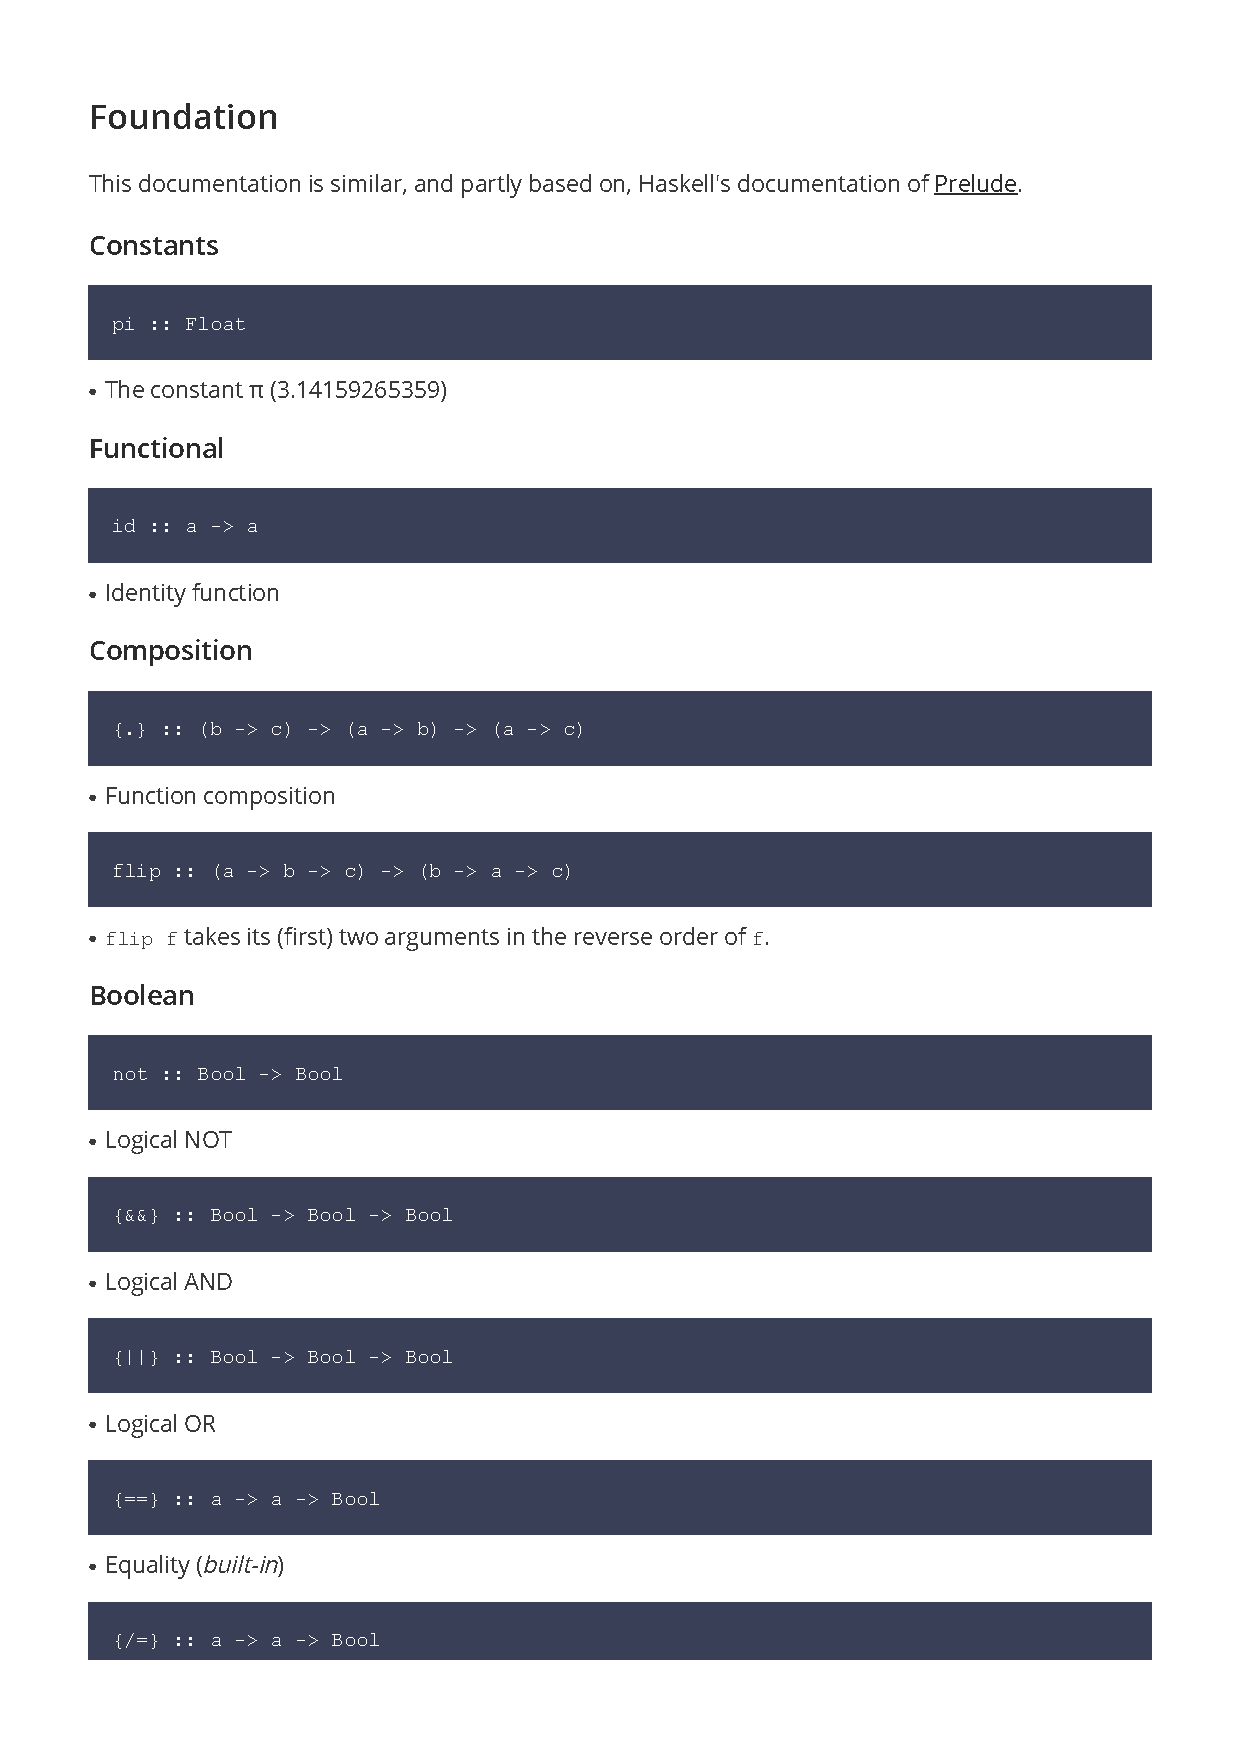
\includepdf[pages=-]{appendices/foundation-doc.pdf}



\end{document}
